\section{Experimental Design} 
\label{sec:Evaluation}

In this section we explain how we empirically evaluate our proposal for automated content transplantation in video games through \ApproachName{}. 
Through this section, we present the research questions that we aim to answer, the evaluation method, and the implementation details.

\subsection{Research Questions}

\ApproachName{} proposes a new angle for PCG, and for this reason we need to assess how it compares to the established practice for search-based PCG (SBPCG)  in the video game field. This motivates our first research question:

\textbf{RQ$_1$: }\textit{How does \simhotep{} perform with respect to the current practice for SBPCG?}

We followed the work by Gallota \etal~\cite{gallotta2022evolving} as a search-based  PCG baseline. Gallota \etal proposed a hybrid Evolutionary Algorithm for generating NPCs. Specifically, their approach combines an L-system with a Feasible Infeasible Two Population Evolutionary Algorithm. We choose Gallota \etal as PCG baseline because (1) this work is specific for spaceships that can play the role of bosses which is comparable to the content of our case study, and (2) it achieves the best state-of-the-art results for this type of content. 

Moreover,  since we propose for the first time the use of simulation as objective function to guide the search for transplantation, \simhotep, it is natural to compare it with the established practice in the software transplantation field, which is constituted by the use of test suite to guide the transplantation. This motivates our second research question:

\textbf{RQ$_2$: }\textit{To what extend using a simulation-based objective function to guide the transplantation is more effective than a test-based one?}

To answer RQ2 we empirically compare \ApproachName{} guided by the simulation-based objective function as described in Section 3.6 (which we refer to as \simhotep{} from now on) with  a test-based variant of \ApproachName{} (called \timhotep{}). \timhotep{} uses an objective function based on the number of test cases that are passed by the transplanted software. 
The reason for comparing this variant is that in traditional software transplantation the best results have been achieved by using the test suite as the objective function. 
\CaseStudy{}'s developers provided us with a test suite relevant to the game, consisting of a total of 243 tests selected based on their domain knowledge. 
Therefore the value of \timhotep{}'s objective function is computed by running each individual through the 243 tests, recording the number of tests passed and normalizing this value in a scale of [0, 1]. An individual which passes the 243 tests will obtain an objective function score of 1, on the contrary if it does not pass any test it will obtain an objective function score of 0.  
As in \simhotep{},  each individual also needs to constitute a valid boss (i.e., solution), receiving a score of 0 if it does not represent a valid one (see Section 3.6).

\subsection{Evaluation Process and Settings}
Figure.~\ref{fig:evaluation} shows an overview of the empirical evaluation we carried out to assess \ApproachName{} for the \CaseStudy's case study. The white background part at the top shows the assets of the game itself (content) and the game development (test suite) that are used by the approaches. The grey background part in the middle shows the inputs and outputs of the three approaches (the two \ApproachName{} variants and the baseline). Finally, the white background part at the bottom shows the evaluation of the results of the approaches.

We used five different hosts (i.e., Vermis, Teuthus, Argos, Orion, and Maia), which are the full set of original bosses from \CaseStudy{}. As donors, \CaseStudy{}'s developers considered all \CaseStudy{}'s scenarios to identify 129 organs. Each host has more than a thousand model elements. Organs have an average of 255 model elements. Each organ was transplanted individually to each boss. Each variant of \ApproachName{} provided a total of 645 new individuals (5 hosts * 129 organs) as output, 645 new individuals from \simhotep{} and 645 individuals from \timhotep{}. In the case of the SBPCG baseline (which relies on the L-system to generate the content instead of transplanting organs), to make it a fair comparison, the baseline was executed 129 times with each one of the 5 different hosts to obtain 645 new individuals. In addition, we executed 30 independent runs (to account for random variation as suggested by Arcuri and Fraser~\cite{arcuri2013parameter}). Hence, we obtain a total of 58050 independent runs (645*3*30).

We chose the parameters shown in Table~\ref{tab:evaluation_parameters} to calibrate  \ApproachName{}. We established the stop condition at 2 minutes and 30 seconds, ensuring that the approaches run long enough to obtain suitable solutions. The focus of this paper is not to tune the values to improve the performance of the approaches when applied to a specific problem, but rather to compare their performance in terms of solution quality on a level playing field. 
The implementation uses the Java(TM) SE Runtime Environment (JDK 1.8) and Java as the programming language. All experiments were run using two PCs with the following specifications: Intel Core i7-8750H, 16GB; and  2x Intel(R) Xeon(R) CPU X5660, 64GB.

For purposes of replicability and extension of our work, the source code and the data are publicly available at \url{https://anonymous.4open.science/r/Imhotep/}.

\begin{table}[tb]
	\centering    
	\caption{\ApproachName{} parameter settings}
	\resizebox{.45\columnwidth}{!}{
		\begin{tabular}{ll}
			\hline
			\bf{Parameter description}            & \bf{Value}  \\ \hline
			Stop Criterion                   & 2m 30s \\
			Population size                  & 100    \\
			Number of parents                & 2      \\
			Number of offspring              & 2      \\
			Crossover probability            & 1      \\
			Mutation probability             & 1/150 \\ \hline
		\end{tabular}
	}
	\label{tab:evaluation_parameters}
\end{table}


\begin{figure}[tb]
    \centering
    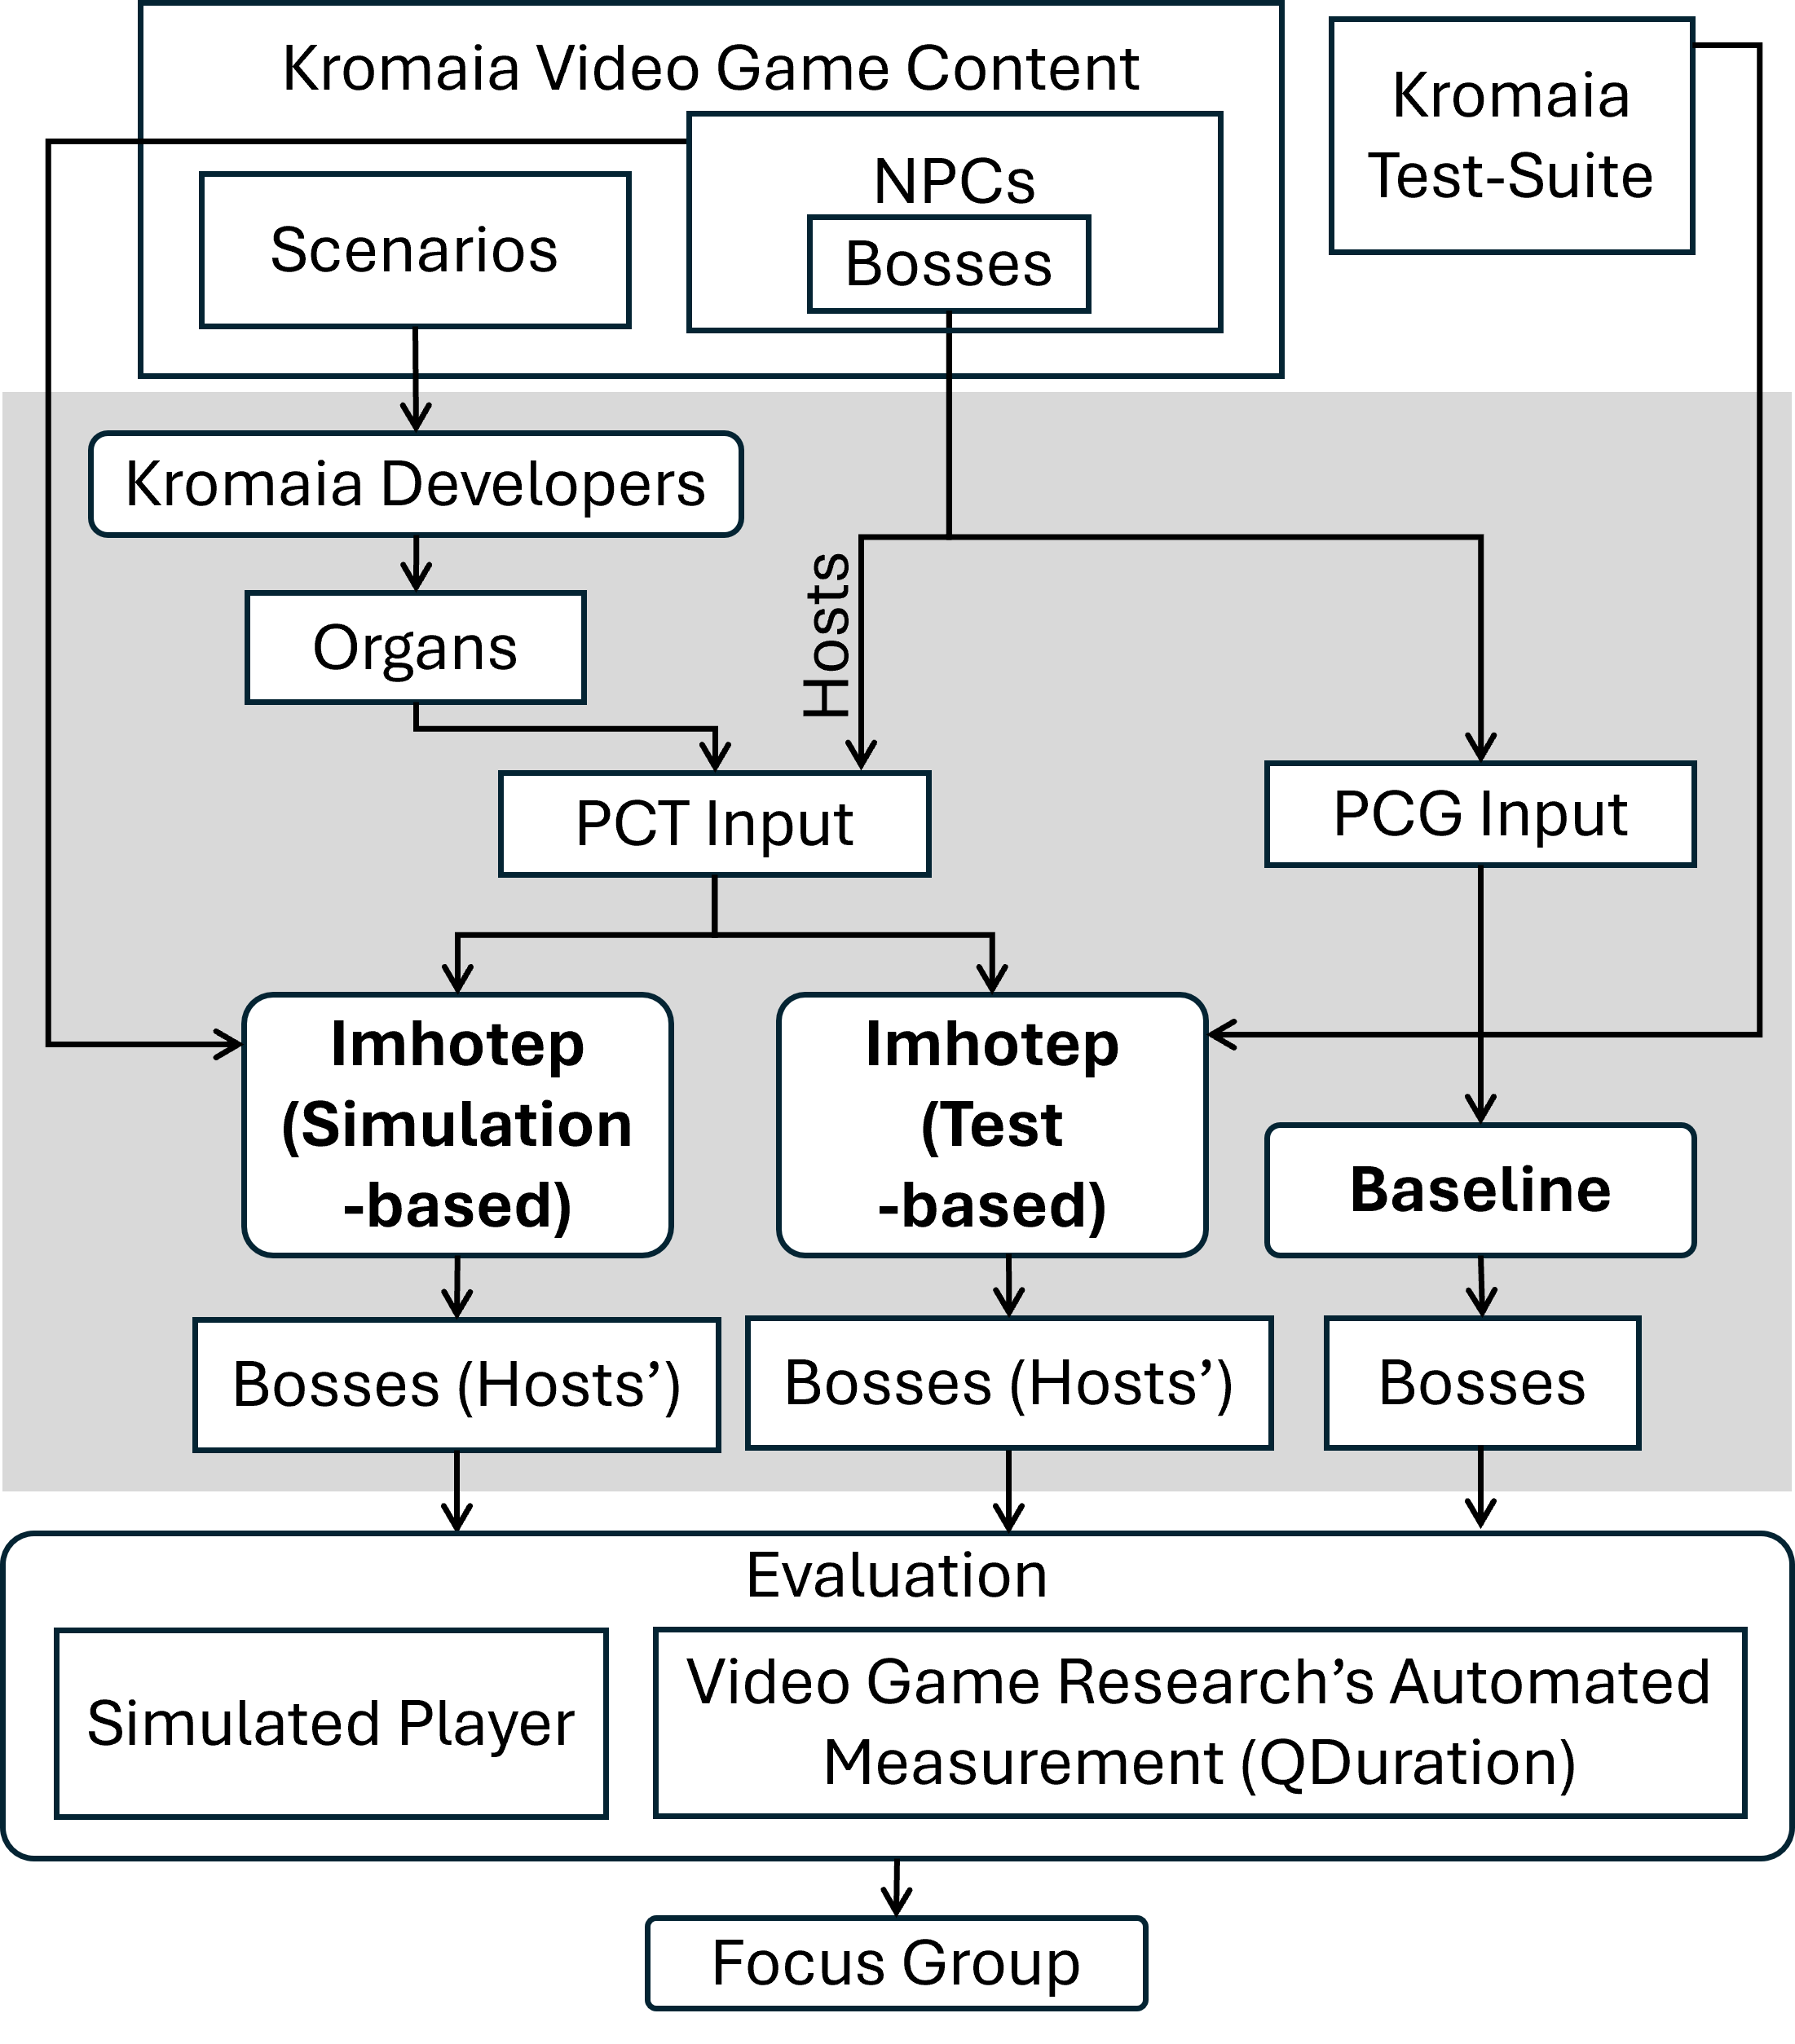
\includegraphics[width=0.3\textwidth]{Figures/evaluation_process.png}
    \caption{Overview of the evaluation process.}
    \label{fig:evaluation}
\end{figure}

\subsection{Evaluation Measures and Statistical Analysis}

To compare the solutions provided by the SBPCG baseline and the two variants of \ApproachName{} (\simhotep{} and \timhotep{}), we rely on the concept of game quality and its automated measurement through simulated players. The results by Browne \etal demonstrated the validity of this approach, which is now widely accepted in the research community~\cite{browne2010evolutionary}. Therefore, we need two ingredients to run our experiment: The simulated player and the automated measurement.

The simulated player, developed by the developers of  \CaseStudy{}, possesses the ability to mimic human player behaviour. Our approach incorporates their algorithm, utilizing it to simulate battles between the generated bosses and the simulated player. Within these simulations, the simulated player confronts the boss, strategically targeting and destroying its weak points. Meanwhile, the boss operates in accordance with its anatomical structure, behavioural patterns, and attack/defensive dynamics, aiming to overcome the simulated player. Both entities within the simulation actively strive to emerge victorious, eschewing draws or ties, and ensuring a definitive win. 
%The algorithm grants the simulated player the capability to employ various strategies when engaging with a boss, as it can be parametrised to define its fighting approach. The simulation parameters were provided by the developers, who analysed battles between human players and bosses to inform their decision-making.

The automated measurement is $Q_{Duration}$ which was proven to achieve good results~\cite{browne2010evolutionary}. The duration of duels between simulated players and bosses units is expected to be around a certain optimal value. For the \CaseStudy{} case study, through tests and questionnaires with players, the developers determined that concentration and engagement for an average boss reach their peak at approximately 10 minutes ($T_{Optimal}$), whereas the maximum accepted time was estimated to be 20 minutes ($2*T_{Optimal}$). Significant deviations from that reference value are good design-flaw indicators: short games are probably too easy; and duels that go on a lot longer than expected tend to make players lose interest. The criterion $Q_{Duration}$ is a measure of the average difference between the duration of each duel ($T_{d}$) and the desired, optimal duration ($T_{Optimal}$):

\begin{equation}
    Q_{Duration} =  1 - \frac{\sum\limits_{d=1}^{Duels}\frac{\mid T_{Optimal} - T_{d} \mid}{T_{Optimal}}}{Duels} 
\end{equation}

Based on the equation above, the higher the $Q_{Duration}$ achieved by a given approach, the better the solutions it produced.

In order to measure whether there is any statistical significance difference between the results obtained by the different approaches we perform the Mann-Whitney U~\cite{mann1947test} setting the confidence limit, $\alpha$, at 0.05, and applying the Bonferroni correction ($\alpha/K$, where K is the number of hypotheses) when multiple hypotheses are tested.  
Unlike parametric tests, the Mann-Whitney U raises the bar for significance, by making no assumptions about underlying data distributions. We performed a one-sided test since we are interested in knowing if our proposed approach, \simhotep{}, would be better than the others. In such a case, the one-sided p-value interpretation would be straightforward. Specifically, for RQ1 we test the following null hypothesis: \textit{The distribution of $Q_{Duration}$ values produced by  \simhotep{}  is better (i.e., higher) than that produced by the SBPCG baseline}.
If the test rejects the Null Hypothesis, the alternative hypothesis would be accepted: \textit{The distribution of $Q_{Duration}$ values produced by \simhotep{} is not better (i.e., not higher) than that produced by the SBPCG baseline}.

Similarly for RQ2 we test the following null hypothesis: \textit{The distribution of $Q_{Duration}$ values produced by  \simhotep{}  is better (i.e., higher) than that produced by \timhotep{}.}
If the test rejects the Null Hypothesis, the alternative hypothesis would be accepted:
\textit{The distribution of $Q_{Duration}$ values produced by \simhotep{}  is not better (i.e., not higher) than that produced by \timhotep{}}.

Moreover, we used effect size to assess whether the statistical significance has practical significance effect size~\cite{Arcuri2014}. To this end we use the Vargha and Delaney's Â$_{12}$ non-parametric effect size measure, as it is recommended to use a standardised measure rather than a pooled one like the Cohen's $d$ when not all samples are normally distributed~\cite{Arcuri2014}, as in our case. 
The Â$_{12}$ statistic measures the probability that an algorithm $A$ yields greater values for a given performance measure $M$ than another algorithm $B$, based on the following equation: 

\begin{equation}
	\hat{A}_{12} = (R_1/m - (m + 1)/2)/n 
\end{equation}

\noindent where $R_1$ is the rank sum of the first data group we are comparing, and $m$ and $n$ are the number of observations in the first and second data sample, respectively. Values between $(0.44, 0.56)$ represent negligible differences, values between $[0.56, 0.64)$ and $(0.36, 0.44]$ represent small differences, values between $[0.64, 0.71)$ and $(0.29, 0:44]$ represent medium differences, and values between $[0.0, 0.29]$ and $[0.71, 1.0]$ represent large differences.

%\subsection{Implementation details}

% \subsection{Quality measurements}
% \label{subsec:Measurements}

% In a recent research done by Browne et al., the experimentation with game users showed that the following criteria stand out as being the most important: Completion, Duration, Uncertainty, Killer Moves, Permanence, and Lead Change \cite{browne2010evolutionary}. Our evaluation measures these criteria with values in the interval [0,1].

% {\bf Completion (Viability):} A game against a boss unit should end with more conclusions (victories for either the player or the boss) than draws/ties. The criterion $Q_{Completion}$ calculates a ratio of conclusions over total duel count:
% \begin{equation}
% Q_{Completion} = \frac{Conclusions}{Duels}
% \end{equation}

%  {\bf Uncertainty (Quality):} In order to keep players engaged with a duel, neither the player nor the boss unit should get extremely close to victory or defeat too early before the duel is settled, with ($T_{d}$) being its duration. Therefore, a duel is considered to be more uncertain the longer the time until the player's or the boss unit's health levels reach a dangerous/critical status ($P_{d}$ and $B_{d}$, respectively). For each duel, $Q_{Uncertainty}$ measures the average deviation between the time at which it is detected that one of the contenders is on the verge of defeat and the time corresponding to the duration of the duel.
% \begin{equation}
% Q_{Uncertainty} =  1 - \frac{\sum\limits_{d=1}^{Duels}\frac{T_{d} - min\left ( P_{d}, B_{d} \right )}{T_{d}}}{Duels} 
% \end{equation}

% {\bf Killer Moves:}   $Q_{KMoves}$ measures the proportion of killer moves by any contender ($K$), taking into account the moves that are considered to be remarkable highlights ($H$) but that are less important than killer moves. In the video game case study, the developers considered that a highlight move happens when either the boss unit or the player experiences a decrease in health; killer moves are those that make the difference in health between the contenders reach 30\%.
% \begin{equation}
% Q_{KMoves} =  1 - \frac{\sum\limits_{d=1}^{Duels}\frac{K_{d}}{H_{d}}}{Duels} 
% \end{equation}

% {\bf Permanence:} Duels with a high permanence value are games in which the advantages given by significant actions or moves by one of the contenders are unlikely to be immediately reverted by the opponent in terms of dominance. In the video game case study, the developers considered every highlight move and killer move to be meaningful actions, with recovery moves ($R$) being those that quickly cancelled the advantages given by other previous killer or highlight moves. The criterion $Q_{Permanence}$ is measured as follows:
% \begin{equation}
% Q_{Permanence} =  1 - \frac{\sum\limits_{d=1}^{Duels}\frac{R_{d}}{H_{d}+K_{d}}}{Duels} 
% \end{equation}

% {\bf Lead Change:} The lack of lead changes indicates low dramatic value. In the video game case study, the lead is determined at any given moment by considering the contender with the highest health level. This criterion is measured taking into account those highlight or killer moves that cause the lead to change ($L$) during the course of a duel:
% \begin{equation}
% Q_{LChange} = \frac{\sum\limits_{d=1}^{Duels}\frac{L_{d}}{H_{d}+K_{d}}}{Duels} 
% \end{equation}

% $Q_{Overall}$ calculates an average quality value for a model, including all of the quality criterion studied:
% \begin{equation}
% Q_{Overall} = \frac{\sum\limits_{i=1}^{N}Q_{i}}{N}
% \end{equation}